\documentclass[tikz]{standalone}

\usetikzlibrary{calc,positioning,patterns,decorations.pathmorphing,decorations.markings,shapes.geometric}

\tikzset{jagged/.style={%
  -,rounded corners=0.5pt,
  decorate,
  decoration={random steps,segment length=4pt,amplitude=2.5pt},
}}

\def\x{12mm}
\def\y{2.25cm}


\begin{document}

\begin{tikzpicture}[
  every node/.style={draw,fill=black!3,thick, minimum width=5.5cm, minimum height=1cm,align=left},
  arrow/.style={->,thick,>=latex}
]

% Compute coordinates of stacked boxes (back to front)
\foreach \i in {3,2,1} {
  \pgfmathsetmacro{\pct}{15*\i + 3}
  % Round the value (optional, for cleaner output)
  \pgfmathtruncatemacro{\pct}{\pct}
  
  \node (B\i) [fill=gray!\pct] at (0.08*\i,0.08*\i) {};
}

% Draw main node on top
\node (problems) at (0,0) {\textbf{\small Problems}\\{\footnotesize convex optimization, root finding, \ldots}};

\node (alg) [above=5mm of problems.north west, anchor=south west] {\textbf{\small Iterative Numerical Algorithm}\\{\footnotesize gradient descent, bisection,\ldots}};

\coordinate (c) at ($(alg.south east)!0.5!(problems.north east)$);

\node (autoalg) [right=1.5cm of c, anchor=west, inner sep=20pt, align=center, jagged, text width=2cm, minimum width=2cm] {\bfseries Automated\\analysis};

\node [right=1.5cm of autoalg.east, anchor=west, minimum width=0pt] (bound) {\textbf{\small Worst-Case Bound}\\[6pt]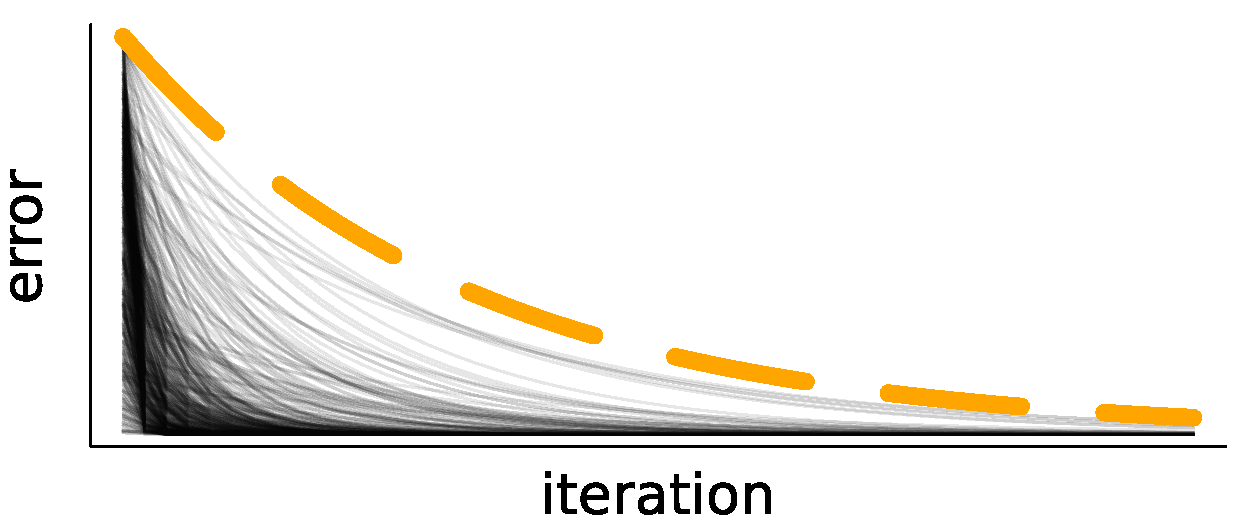
\includegraphics[width=4.1cm]{_code/plot.pdf}};

\draw [arrow] (alg) -- ($(alg -| autoalg.west)-(1mm,0)$);
\draw [arrow] (B3) -- ($(B3 -| autoalg.west)-(1mm,0)$);
\draw [arrow] (autoalg) -- (bound.west);

% \draw [fill=blue] ($(alg.north west)+(0,3mm)$) rectangle ($(alg.north west)+(6.5in,4mm)$);

\end{tikzpicture}

\end{document}
